\documentclass[border=4pt]{standalone}

\usepackage{amsmath}
\usepackage{tikz}
\usepackage{mathdots}
\usepackage{yhmath}
\usepackage{cancel}
\usepackage{color}
\usepackage{siunitx}
\usepackage{array}
\usepackage{multirow}
\usepackage{amssymb}
\usepackage{gensymb}
\usepackage{tabularx}
\usepackage{booktabs}
\usetikzlibrary{fadings}
\usetikzlibrary{patterns}


\begin{document}
 


\tikzset{every picture/.style={line width=0.75pt}} %set default line width to 0.75pt        

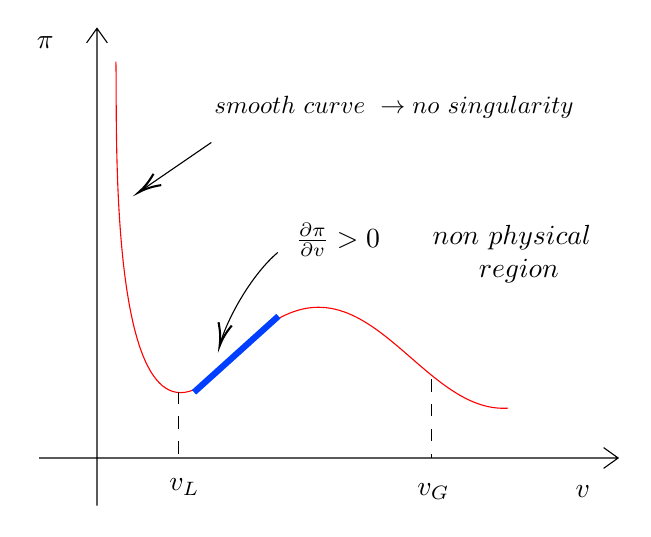
\begin{tikzpicture}[x=0.75pt,y=0.75pt,yscale=-1,xscale=1]
%uncomment if require: \path (0,300); %set diagram left start at 0, and has height of 300

%Shape: Axis 2D [id:dp19348955028335046] 
\draw  (88,238) -- (367,238)(115.9,31) -- (115.9,261) (360,233) -- (367,238) -- (360,243) (110.9,38) -- (115.9,31) -- (120.9,38)  ;
%Curve Lines [id:da1622656876746693] 
\draw [color={rgb, 255:red, 255; green, 0; blue, 0 }  ,draw opacity=1 ]   (125,47) .. controls (126,73) and (119,261) .. (180,191) .. controls (241,121) and (267,217) .. (314,214) ;


%Straight Lines [id:da27057605714347677] 
\draw  [dash pattern={on 4.5pt off 4.5pt}]  (155,206) -- (155,237) ;


%Straight Lines [id:da4904565317065068] 
\draw  [dash pattern={on 4.5pt off 4.5pt}]  (277,200) -- (277,238) ;


%Straight Lines [id:da1349810080997138] 
\draw [color={rgb, 255:red, 0; green, 63; blue, 255 }  ,draw opacity=1 ][line width=2.25]    (162.67,206.33) -- (203.33,169.67) ;


%Curve Lines [id:da5600677416258235] 
\draw    (203,139) .. controls (190.65,149.45) and (179.2,169.83) .. (175.52,182.13) ;
\draw [shift={(175,184)}, rotate = 284.04] [color={rgb, 255:red, 0; green, 0; blue, 0 }  ][line width=0.75]    (10.93,-3.29) .. controls (6.95,-1.4) and (3.31,-0.3) .. (0,0) .. controls (3.31,0.3) and (6.95,1.4) .. (10.93,3.29)   ;

%Straight Lines [id:da6202375716744366] 
\draw    (171,86) -- (137.65,108.87) ;
\draw [shift={(136,110)}, rotate = 325.56] [color={rgb, 255:red, 0; green, 0; blue, 0 }  ][line width=0.75]    (10.93,-3.29) .. controls (6.95,-1.4) and (3.31,-0.3) .. (0,0) .. controls (3.31,0.3) and (6.95,1.4) .. (10.93,3.29)   ;


% Text Node
\draw (91,38) node    {$\pi $};
% Text Node
\draw (350,254) node    {$v$};
% Text Node
\draw (158,252) node    {$v_{L}$};
% Text Node
\draw (278,254) node    {$v_{G}$};
% Text Node
\draw (232,133) node    {$\frac{\partial \pi }{\partial v}  >0$};
% Text Node
\draw (318,140) node    {$ \begin{array}{l}
non\ physical\ \\
\ \ \ \ \ region
\end{array}$};
% Text Node
\draw (259,69) node  [scale=0.9]  {$smooth\ curve\ \rightarrow no\ singularity$};


\end{tikzpicture}

\end{document}
